\newpage
\subsection{Caso d'uso UC19: Iscrizione questionario}
\label{UC19}
\begin{figure}[ht]
\centering
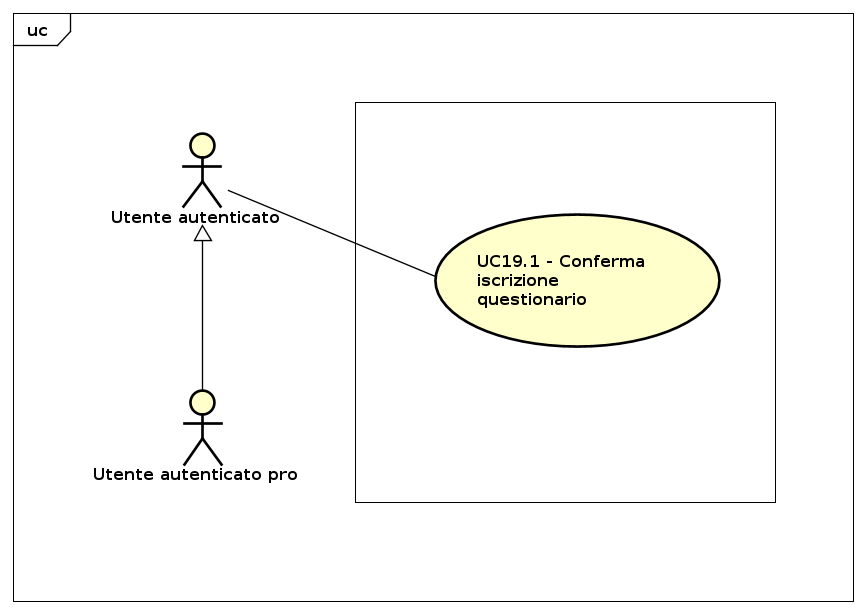
\includegraphics[scale=0.5,keepaspectratio]{UML/UC19.png}
\caption{UC19: Iscrizione questionario}
\end{figure}
\FloatBarrier
\begin{itemize}
\item\textbf{Attori}: utente autenticato, utente autenticato pro;
\item\textbf{Descrizione}: dopo aver ricercato un questionario, l'attore può iscriversi ad esso;
\item\textbf{Precondizione}: l'attore ha utilizzato la barra di ricerca per cercare un questionario ed ha scelto il questionario che vorrebbe svolgere tra i risultati proposti;
\item\textbf{Postcondizione}: l'attore si è iscritto al questionario che ha scelto;
\item\textbf{Scenario principale}:
\begin{enumerate}
\item L'attore può confermare l'iscrizione al questionario (UC19.1).
\end{enumerate} 
\item\textbf{Scenari alternativi}: l'attore cambia idea sul questionario al quale vuole iscriversi e annulla l'operazione tornando alla schermata precedente.
\end{itemize}

\subsubsection{Caso d'uso UC19.1: Conferma iscrizione questionario}
\label{UC19.1}
\begin{itemize}
\item\textbf{Attori}: utente autenticato, utente autenticato pro;
\item\textbf{Descrizione}: l'attore può confermare l'iscrizione al questionario;
\item\textbf{Precondizione}: l'attore si è iscritto ad un questionario;
\item\textbf{Postcondizione}: l'attore ha confermato l'iscrizione al questionario;
\item\textbf{Scenario principale}: l'attore conferma l'iscrizione al questionario.
\end{itemize}